\section{Thursday, April 18th}
\subsection{Logistics}
\begin{itemize}
    \item Discussion post by Sunday
\end{itemize}

\subsection{Goals}
\begin{itemize}
    \item Channel Capacity w/ and w/o feedback
    \item Joint Typicality (+ AEP)
\end{itemize}

\subsection{Channel Coding Theorem}
If a channel $(\cX, \cY)$
\begin{enumerate}
    \item Discrete: $\cX, \cY$ are discrete.
    \item Memoryless: $Y_i\stackrel{\indep}{\text{given } X_i} \text{ of } y^{(i-1)}, x^{(i-1)}$.
\end{enumerate}
then:
\begin{enumerate}
    \item If $R < C$ then $R$ is achievable.
    \begin{shaded}
        Recall: $R$ is achievable if $\exists$ a set of messages $\cW$. prior $p_\cW$, and encoding $\cC$ s.t. $|\cW|=d^{nR}$\\
        $|C(w)|=n$ (strings length $n$) \underline{and} $\lambda^{(n)}=\max_{w\in
        cW}\{\Pr(\what\neq w\mid \cW = w)\}\stackrel{\to}{n\to\infty}0$
    \end{shaded}
    \item If $R$ is achievable, $R\leq C$. 
    \begin{shaded}
        ($R>C$ is \underline{not} achievable)
    \end{shaded}
\end{enumerate}
where $C=\max_{P_x}\left\{I[X; Y]\right\}$.

We showed last time that $C=1-H[E] = 1 - H([p, 1-p])$, where $E$ indicates an error: $X\neq Y$.

\subsection{Relevant Results in this class}
\begin{enumerate}
    \item Chain Rule: 
    \begin{align*}
        H[X, Y] &= H[X]+H[Y \mid X] \\
        H\left[X^{(\mu)}\right] &= \sum_{i=1}^n H\left[X_1 \mid x^{(1-1)}\right]
    \end{align*}
    \item Joint $\leq$ Sum: $\displaystyle H\left[X^{(n)}\right] \leq \sum_{i=1}^n H\left[X_i\right]$
    \item Data Processing: $X \rightarrow Y \rightarrow W$ then $I[X ; W] \leq I[X ; Y]$
    \item Fano's Inequality: $H[X \mid \hat{x}] \leq 1+P_r(X \neq \hat{x}) \log (|\cX|)$
    \item Conditioning $\searrow$ Uncertainty: $H[X \mid Y] \leq H[X]$ 
    (w/ equality if $\indep$)
\end{enumerate}

\begin{figure}[h]
    \centering
    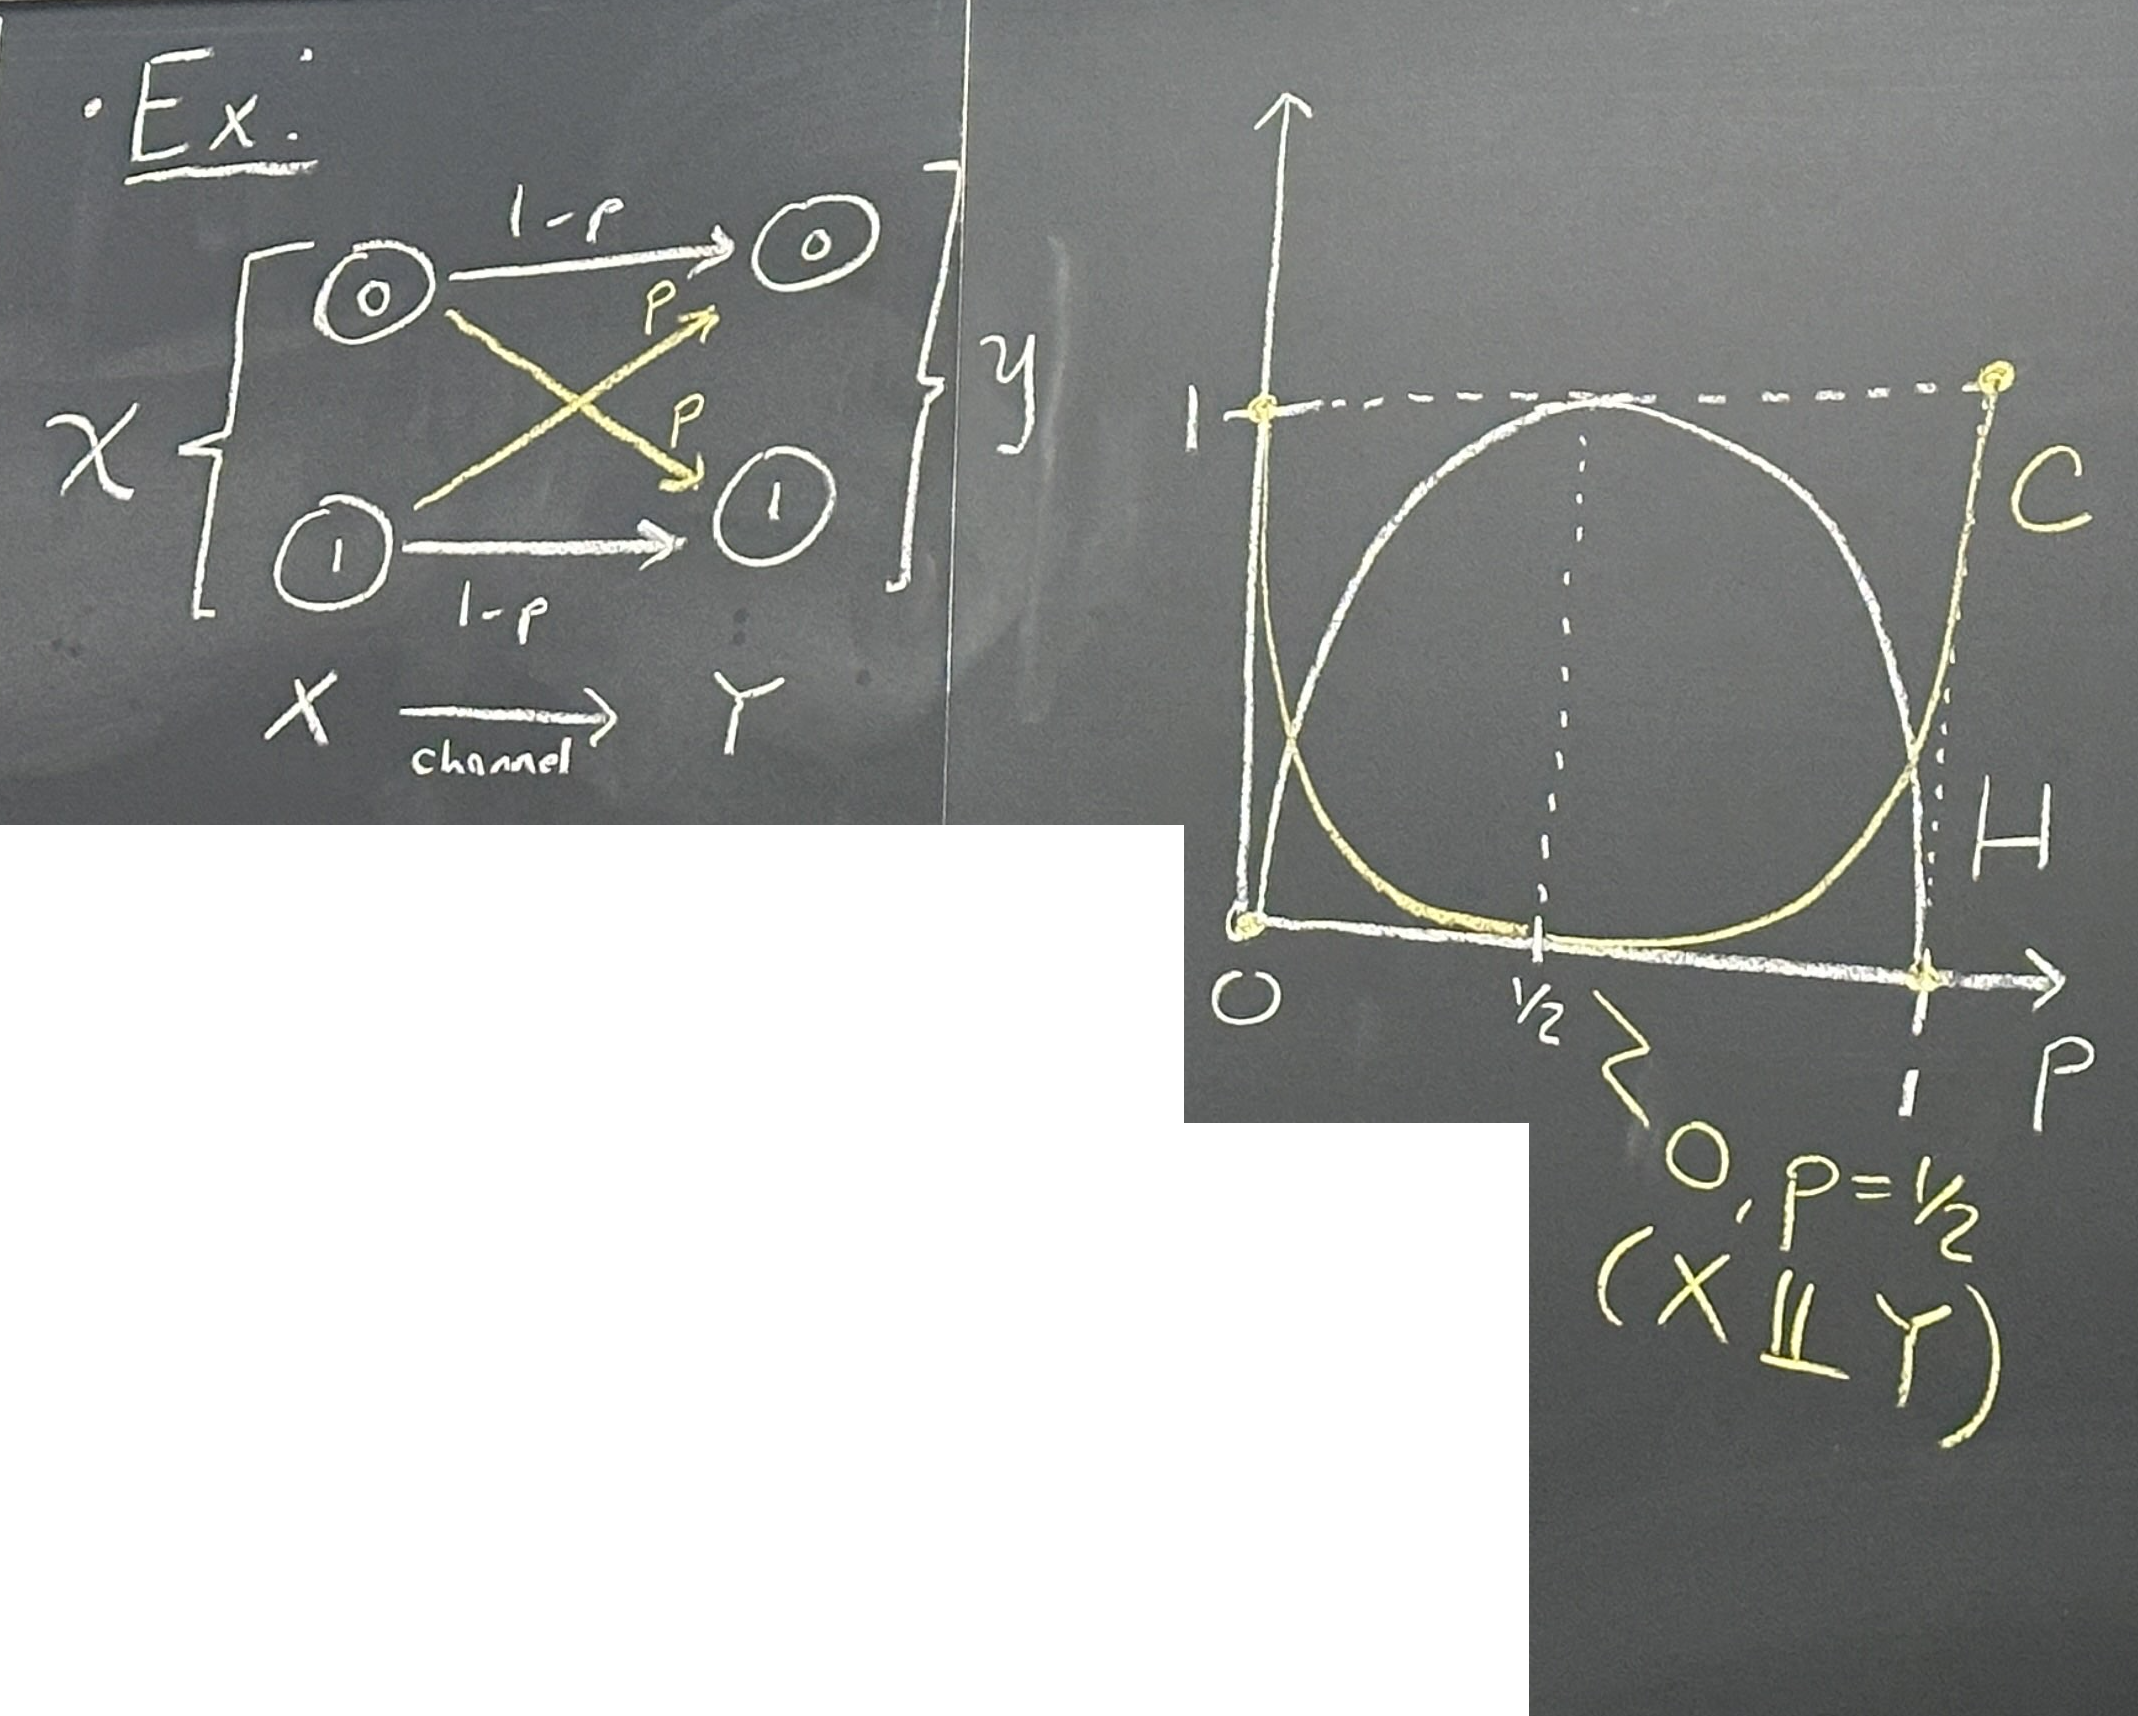
\includegraphics[scale=0.14]{lectures/wk13/img/capacity.png}
    % \caption{Channel Capacity}
    \label{fig:capacity}
\end{figure}

\subsection{The Feedback Capacity Theorem (7.12)}
A channel with feedback is illustrated in the first lecture for this class. We assume that all the received symbols are sent back immediately and noiselessly to the transmitter, which can then use them to decide which symbol to send next. Can we do better with feedback? The surprising answer is no, which we shall now prove. We define a $\left(2^{n R}, n\right)$ feedback code as a sequence of mappings $x_i\left(W, Y^{i-1}\right)$, where each $x_i$ is a function only of the message $W \in 2^{n R}$ and the previous received values, $Y_1, Y_2, \ldots, Y_{i-1}$, and a sequence of decoding functions $g: \mathcal{Y}^n \rightarrow\left\{1,2, \ldots, 2^{n R}\right\}$. Thus,
$$
P_e^{(n)}=\operatorname{Pr}\left\{g\left(Y^n\right) \neq W\right\},
$$
when $W$ is uniformly distributed over $\left\{1,2, \ldots, 2^{n R}\right\}$.
Definition The capacity with feedback, $C_{\mathrm{FB}}$, of a discrete memoryless channel is the supremum of all rates achievable by feedback codes.

Theorem 7.12.1 (Feedback capacity)
$$
C_{\mathrm{F} B}=C=\max _{p(x)} I\left[X ; Y\right].
$$

\begin{Answer}
Proof: Since a nonfeedback code is a special case of a feedback code, any rate that can be achieved without feedback can be achieved with feedback, and hence
$$
C_{\mathrm{FB}} \geq C.
$$

Proving the inequality the other way is slightly more tricky. We cannot use the same proof that we used for the converse to the coding theorem without feedback. Lemma 7.9.2 is no longer true, since $X_i$ depends on the past received symbols, and it is no longer true that $Y_i$ depends only on $X_i$ and is conditionally independent of the future $X$ 's in (7.93).
\end{Answer}

This essentially states that the Channel Coding Thm. is true w/ feedback.

\subsection{Joint Typicality}
Defn.: given $\left(X^{(n)}, Y^{(n)}\right)$, i.i.d from $P_{x^n, Y^n}$ where $P_{x^n, Y^{(n)}}\left(X^{(n)}, Y^{(n)}\right)=\prod_{i=1}^n P_{x, y}\left(x_i, y_i\right)$
\begin{enumerate}
    \item[(i)] $X^{(n)}$ is typical w.r.t.
and $-\frac{1}{n} \log \left(p_{x^n}\left(x^{(n)}\right)\right) \in H L x$ typical w.r.t. $P_y$:
$$
-\frac{1}{n} \log \left(p_{x^n, r^n}\left(x^{(n)}, Y^{(n)}\right)\right) \in H[X, Y] \pm \varepsilon .
$$
\underline{and}
    \item[(iii)] $\left(X^{(n)}, Y^{(n)}\right)$ is typical w.r.t. $p_X$
\end{enumerate}

\begin{figure}[h]
    \centering
    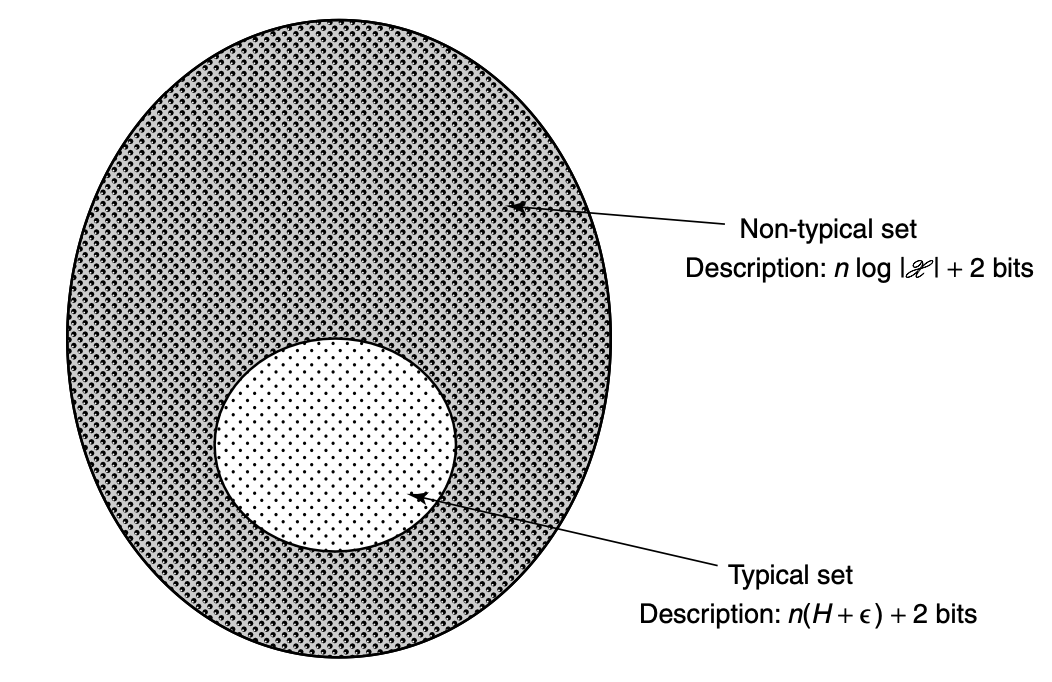
\includegraphics[scale=0.6]{lectures/wk13/img/typical_sets.png}
    \caption{Source code using the typical set shows the Typical set is smaller than any Non-typical set.}
    \label{fig:typical-sets}
\end{figure}

\subsection{Joint AEP}
\begin{enumerate}
\item[(i)] (almost all joint seq. are typical jointly (equipartition))
\begin{equation}
\lim_{n \to \infty} P\left(\left(X^n, Y^n\right) \in A_{\varepsilon}^{(n)}\right) 
= 1. 
\end{equation}

\item[(ii)] $P\left(\left(X^n, Y^n\right) = \left(x^n, y^n\right)\right) \in \leq 2^{-n(H[X,Y]\pm\varepsilon)}, \quad \left(x^n, y^n\right)\in A_{\varepsilon}^n$.

\item[(iii)] 
\begin{align}
\left|A_{\varepsilon}^{(n)}\right| 
    &\leq 2^{n(H[X,Y]+\varepsilon)}
\quad\forall n &&[\text{size is relatively small}]
\\
&\geq (1-\delta)2^{n(H(X,Y)-\varepsilon)}
&&[\text{for $n$ large}]
\end{align}

\item[(iv)] If $\tilde{X}^{(n)}\sim P_{X^n}, \tilde{Y}^{(n)} \sim P_{Y^n}, \tilde{X}^{(n)} \text{ is typical is } \indep \text{ of $\tilde{Y}^{(n)}$ being typical, per (i) and (ii) above: }$ 
\begin{align}
P\left(\left(\tilde X^{(n)}, \tilde Y^{(n)}\right) \in A_{\varepsilon}^{(n)}\right) &\leq 2^{-n(I[X;Y]-3\varepsilon)} \quad &&\forall n 
\\
&\geq (1-\varepsilon)2^{-n(I[X;Y]+3\varepsilon)} \quad &&\text{for } n \text{ large}. 
\end{align}
\end{enumerate}


\subsection{Constructing inequalities}
\begin{itemize}
    \item \# messages: $2^{n R}, \quad$ where $R=\frac{\log_2(|\cW|)}{n}$
    \item Given $X^{(n)}=x^{(n)}: 2^{n H[Y \mid X]}$
    \item Across $2^{n H[Y]} \quad$ typical outcomes
    \begin{align}
    2^{n R} \cdot 2^{n H[Y \mid X]} 
        &\leq 2^{n H[Y]} \\
    R+H[Y \mid X] \leq H[Y], \ 
    &
    R \leq I[X ; Y] \leq C.
    \end{align}
\end{itemize}

\begin{figure}[h]
    \centering
    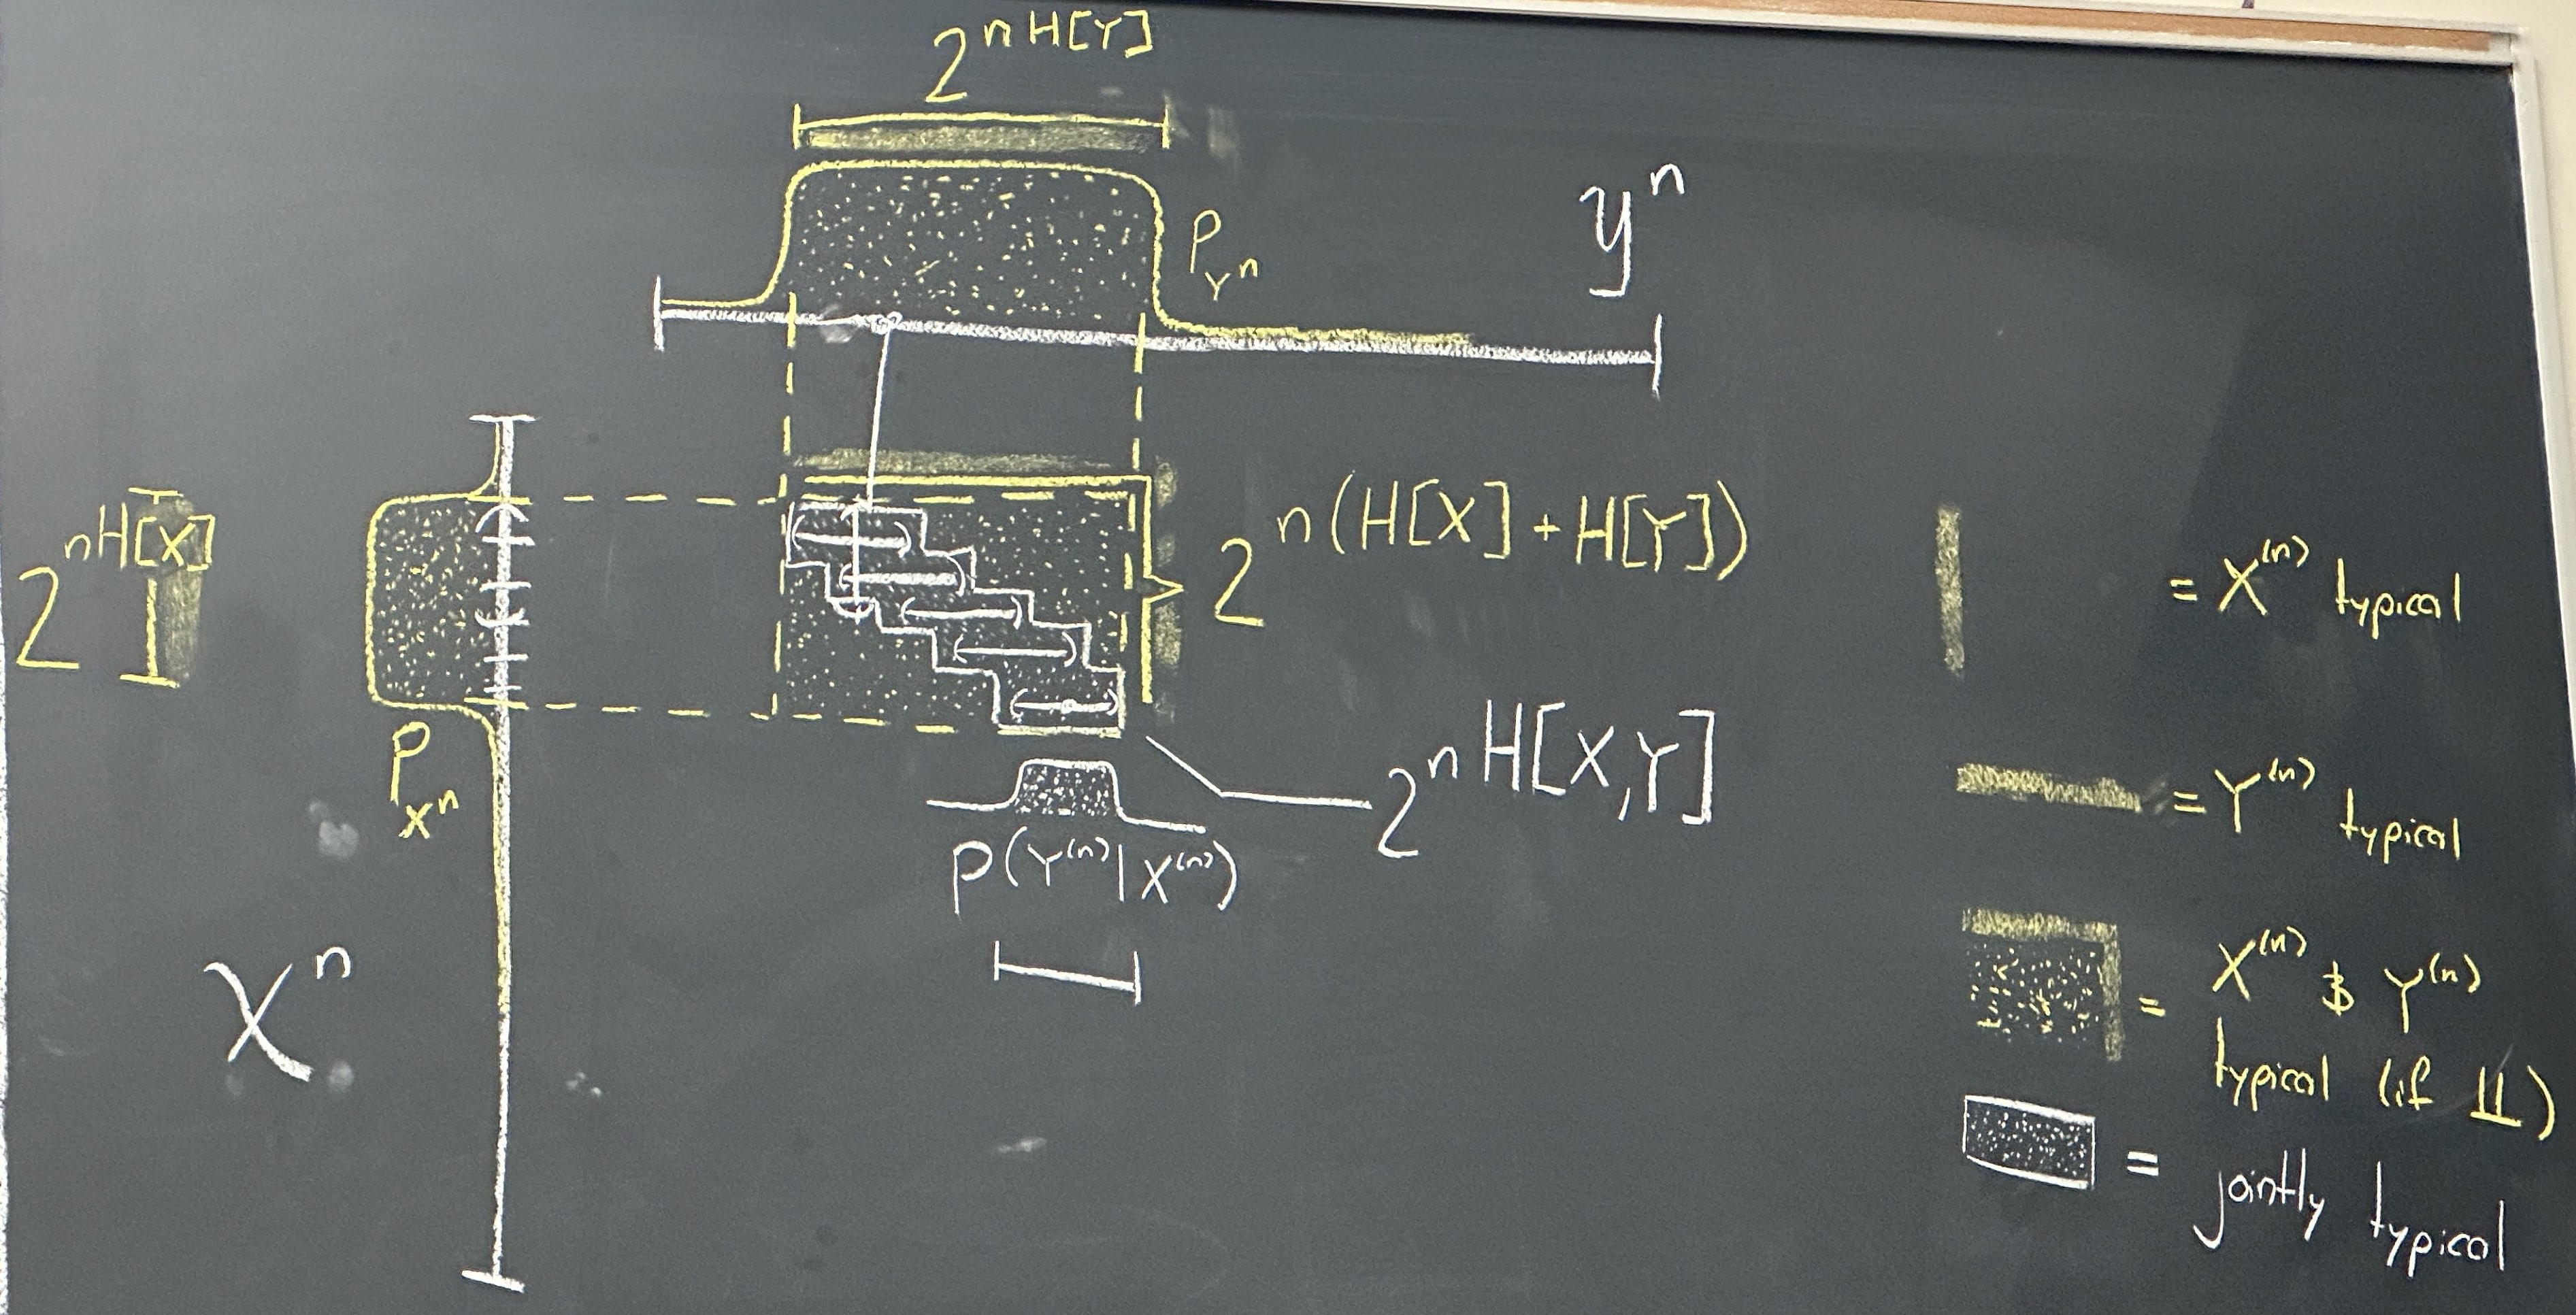
\includegraphics[scale=0.1]{lectures/wk13/img/strip.jpg}
    % \caption{Diagonal Strip}
    \label{fig:strip_firsttime}
\end{figure}

\subsection{Proving that our packing argument is tight}
2. If $R>C$, then $R$ is \underline{not} achievable.\\
If $R$ is achievable then $R \leq C$.
\begin{itemize}
    \item $R$ is achievable $\implies $
    \item Then $P_e^{(i)}=\frac{1}{|\cW|} \sum_w P_r(\hat{w} \neq w \mid W=w) \leq \lambda^{(n)} \longrightarrow 0$
    \begin{itemize}
        \item Consider a model where $W \sim\Uniform({\cW})$
    \begin{equation}
    P_e^{(n)}=\operatorname{Pr}(\hat{w} \neq w) 
    \stackrel{\rightarrow}{{n \rightarrow \infty}}
    0
    \end{equation}
        \item $\implies R \leq C$.
    \end{itemize}
\end{itemize}

\subsection{Putting together Past Relevant Results}
\begin{flalign*}
nR &= \log(|\mathcal{W}|) = H[W] = H\left[W|\What\right] + I\left[W;\What\right] \\
&\leq 1 + P_e^{(n)} \log(|\mathcal{W}|) + I[W;\What] 
&&[\text{Fano's Inequality}]
\\
&= 1 + \underbrace{P_e^{(n)}}_{\to 0 \text{ as } n\to\infty}nR + I[W;\What]
\end{flalign*}
\begin{flalign*}
I\left[W;\underbrace{\What}_{g(Y^{(n)})}\right]
&\leq I\left[W;\hat{Y}^{(n)}\right] = 
H\left[W\right] 
- 
H\left[W|Y^{(n)}\right] 
&&[\text{Data Processing Inequality}] \\
&= I\left[\hat{Y}^{(n)};W\right] 
= H\left[\hat{Y}^{(n)}\right] - H\left[\hat{Y}^{(n)}|W\right]
\end{flalign*}
\begin{flalign*}
H\left[\hat{Y}^{(n)}|W\right] 
&= H\left[Y_1, Y_2, \ldots Y_n \mid W\right] \\
&= \sum_{i=1}^{n} H\left[Y_i^{(n)}|Y^{(i-1)},W\right] &&[\text{Chain Rule}] \\
&=\sum_{i=1}^n H\left[Y_i \mid X_i\right]\\
X_i &= \text{function}(Y^{(i-1)},W) &&[\text{Feedback}] \\
H[Y_i|Y^{(i-1)}, W, X_i] &= H[Y_i \mid X_i] &&[\text{Memoryless}]
\end{flalign*}


